%========================================
% LESSON CONTENT: Valor Absoluto y Leyes de Signos
%========================================

\lesson{Valor Absoluto y Leyes de Signos}

\subsectiontitle{Valor Absoluto}

\subsection{Definición}

\begin{definition}
El \textbf{valor absoluto} de un número real $a$, denotado $|a|$, se define como sigue:

$$|a| = \begin{cases}
a & \text{si } a \geq 0 \\
-a & \text{si } a < 0
\end{cases}$$
\end{definition}

\subsection{Interpretación Geométrica}

En general tenemos:

$$|a| = |-a|$$

En una recta coordenada, la distancia entre un punto con coordenada $a$ al origen es la misma que la distancia del punto con coordenada $-a$ al origen.

\subsection{Ejemplo Visual en la Recta Numérica}

\begin{center}
\shorthandoff{<>}
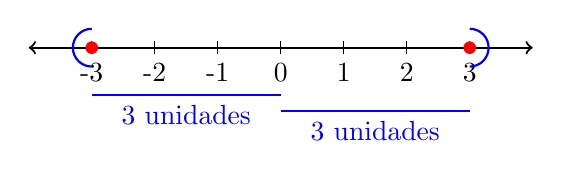
\begin{tikzpicture}[scale=0.8]
    % Draw number line
    \draw[thick, <->] (-4,0) -- (4,0);
    
    % Mark integers
    \foreach \x in {-3,-2,-1,0,1,2,3}
        \draw (\x,0.1) -- (\x,-0.1) node[below] {\x};
    
    % Highlight -3 and 3
    \fill[red] (-3,0) circle (0.1);
    \fill[red] (3,0) circle (0.1);
    
    % Draw distance arcs
    \draw[blue, thick] (-3,0.3) arc (90:270:0.3);
    \draw[blue, thick] (3,0.3) arc (90:-90:0.3);
    
    % Distance lines to origin
    \draw[blue, thick] (-3,-0.75) -- (0,-0.75) node[midway, below] {3 unidades};
    \draw[blue, thick] (0,-1.0) -- (3,-1.0) node[midway, below] {3 unidades};
\end{tikzpicture}
\shorthandon{<>}
\end{center}

$$|-3| = |3|$$

\begin{itemize}
    \item La distancia entre $-3$ y el origen es de 3 unidades.
    \item La distancia entre $3$ y el origen es de 3 unidades.
\end{itemize}

Por lo tanto: $|-3| = |3| = 3$

\subsectiontitle{Ejemplos de Valor Absoluto}

\textbf{Instrucción:} Reescribe el número sin usar el símbolo de valor absoluto, y simplifica el resultado.

\begin{example}
\textbf{Ejemplo 1}
$$|-11 + 1| = |-10| = -(-10) = 10$$

\textbf{Explicación paso a paso:}
\begin{enumerate}
    \item Primero resolvemos dentro del valor absoluto: $-11 + 1 = -10$
    \item Aplicamos la definición de valor absoluto: como $-10 < 0$, entonces $|-10| = -(-10)$
    \item Simplificamos: $-(-10) = 10$
\end{enumerate}
\end{example}

\begin{example}
\textbf{Ejemplo 2}
$$|6| - |-3| = 6 - 3 = 3$$

\textbf{Explicación paso a paso:}
\begin{enumerate}
    \item $|6| = 6$ (porque $6 \geq 0$)
    \item $|-3| = 3$ (porque $-3 < 0$, entonces $|-3| = -(-3) = 3$)
    \item Por lo tanto: $6 - 3 = 3$
\end{enumerate}
\end{example}

\begin{example}
\textbf{Ejemplo 3}
$$|8| + |-9| = 8 + 9 = 17$$

\textbf{Explicación paso a paso:}
\begin{enumerate}
    \item $|8| = 8$ (porque $8 \geq 0$)
    \item $|-9| = 9$ (porque $-9 < 0$, entonces $|-9| = -(-9) = 9$)
    \item Por lo tanto: $8 + 9 = 17$
\end{enumerate}
\end{example}

\subsectiontitle{Propiedades de Signos}

Las siguientes propiedades son fundamentales para trabajar con números negativos y operaciones algebraicas:

\begin{center}
\begin{tabular}{|l|l|}
\hline
\textbf{Propiedad} & \textbf{Ejemplo} \\
\hline
$(-1)a = -a$ & $(-1)8 = -8$ \\
\hline
$-(-a) = a$ & $-(-6) = 6$ \\
\hline
$(-a)b = a(-b) = -(ab)$ & $(-2)3 = 2(-3) = -(2 \cdot 3)$ \\
\hline
$(-a)(-b) = ab$ & $(-7)(-8) = 7 \cdot 8$ \\
\hline
$-(a + b) = -a - b$ & $-(4 + 9) = -4 - 9$ \\
\hline
$-(a - b) = b - a$ & $-(3 - 5) = 5 - 3$ \\
\hline
\end{tabular}
\end{center}

\subsection{Explicación Detallada de las Propiedades}

\subsubsection{Propiedad del Factor -1}
$$(-1)a = -a$$

Multiplicar cualquier número por $-1$ es equivalente a cambiar su signo.

\textbf{Ejemplo:} $(-1) \cdot 8 = -8$

\subsubsection{Doble Negación}
$$-(-a) = a$$

El negativo del negativo de un número es el número original.

\textbf{Ejemplo:} $-(-6) = 6$

\subsubsection{Distributividad del Signo Negativo en Productos}
$$(-a)b = a(-b) = -(ab)$$

Un signo negativo puede ``moverse'' entre los factores de un producto.

\textbf{Ejemplo:} $(-2) \cdot 3 = 2 \cdot (-3) = -(2 \cdot 3) = -6$

\subsubsection{Producto de Dos Números Negativos}
$$(-a)(-b) = ab$$

El producto de dos números negativos es positivo.

\textbf{Ejemplo:} $(-7) \cdot (-8) = 7 \cdot 8 = 56$

\subsubsection{Distributividad del Signo Negativo en Sumas}
$$-(a + b) = -a - b$$

El negativo de una suma es igual a la suma de los negativos.

\textbf{Ejemplo:} $-(4 + 9) = -4 - 9 = -13$

\subsubsection{Distributividad del Signo Negativo en Restas}
$$-(a - b) = b - a$$

El negativo de una resta invierte el orden de los términos.

\textbf{Ejemplo:} $-(3 - 5) = 5 - 3 = 2$

\subsection{Reglas de Signos para Operaciones}

\textbf{Multiplicación y División:}
\begin{itemize}
    \item $(+) \times (+) = (+)$
    \item $(+) \times (-) = (-)$
    \item $(-) \times (+) = (-)$
    \item $(-) \times (-) = (+)$
\end{itemize}

\textbf{Suma y Resta:}
\begin{itemize}
    \item Para sumar números con el mismo signo: suma los valores absolutos y conserva el signo común
    \item Para sumar números con signos diferentes: resta los valores absolutos y conserva el signo del número con mayor valor absoluto
    \item Para restar: cambia el signo del sustraendo y suma
\end{itemize}

\subsection{Ejemplos de Aplicación}

\begin{example}
\begin{enumerate}
    \item \textbf{Multiplicación:} $(-3) \times (-4) = 12$
    \item \textbf{División:} $(-15) \div (-3) = 5$
    \item \textbf{Suma con signos iguales:} $(-7) + (-3) = -10$
    \item \textbf{Suma con signos diferentes:} $(-8) + 5 = -3$
    \item \textbf{Resta:} $7 - (-3) = 7 + 3 = 10$
\end{enumerate}
\end{example}

\subsectiontitle{Resumen de Conceptos Clave}

\begin{enumerate}
    \item \textbf{Valor Absoluto:} Siempre es no negativo y representa la distancia al origen
    \item \textbf{Propiedades de Signos:} Permiten manipular expresiones algebraicas con números negativos
    \item \textbf{Aplicaciones:} Fundamentales para resolver ecuaciones y simplificar expresiones algebraicas
\end{enumerate}

Estas herramientas son esenciales para el álgebra y forman la base para conceptos más avanzados en matemáticas.